%%%%%%%%%%%%%%%%%%%%%%%%%%%%%%%%%%%%%%%
%%% MG 28/12/2018 - Technical notes %%%
%%%%%%%%%%%%%%%%%%%%%%%%%%%%%%%%%%%%%%%

%%%% Preamble %%%%
\documentclass[a4paper]{article}

% wider text, smaller margins
\usepackage{a4wide}

\usepackage[T1]{fontenc}
\usepackage{kpfonts}

%% loads amsmath and some extra
%\usepackage{mathtools}
%\usepackage{amssymb}

% for hyperrefs
\usepackage{hyperref}

% for proofs
\usepackage{amsthm}
% for indicator func
\usepackage{bbm}

% shorthand formats for vector and matrix
\newcommand{\vc}[1]{\mathbf{#1}}%%
\newcommand{\nn}{\nonumber \\}%

% argmin/max opearator
\DeclareMathOperator*{\argmin}{arg\,min}%
\DeclareMathOperator*{\argmax}{arg\,max}%
\DeclareMathOperator{\tr}{tr}
% shortands for common math
\newcommand{\mR}{\mathbb{R}}%% real numbers
\newcommand{\mN}{\mathbb{N}}%% natural numbers

\newcommand{\bx}{\mathbf{x}}%%
\newcommand{\bw}{\mathbf{w}}%%
\newcommand{\bz}{\mathbf{z}}%%

\newcommand{\mD}{\mathcal{D}}%% data space
\newcommand{\mG}{\mathcal{G}}%% sub-Gaussian r.v.
\newcommand{\mS}{\mathcal{S}}%% sigma algebra
\newcommand{\mT}{\mathcal{T}}%% sigma algebra
\newcommand{\mX}{\mathcal{X}}%% input space
\newcommand{\mY}{\mathcal{Y}}%% output space
\newcommand{\mZ}{\mathcal{Z}}%% input-output space

\newcommand{\rE}{\mathrm{E}}%% expectation
\newcommand{\rP}{\mathrm{P}}%% probability
\newcommand{\ind}{\mathbbm{1}}%% indicator funciton


% MG: quick tool for comments, set showComments to 0 in final version
% define new if
\newif\ifShowComments
% pick one of these two
\ShowCommentstrue % or
%\ShowCommentsfalse
% You may want to put your initials into the text of the notes. e.g \note{MG: this is a note}
\newcommand{\note}[1]{\ifShowComments {\emph{\textbf{Note:} #1}} \else {} \fi}%
\newcommand{\idea}[1]{\ifShowComments {\emph{\textbf{\color{red}Idea:} #1}} \else {} \fi}%
\newcommand{\todo}[1]{\ifShowComments {\color{red}\emph{Todo: #1}} \else {} \fi}%

% for coloring
\usepackage{xcolor}

% Number equations within a section
\numberwithin{equation}{section}

% for index list
\usepackage{makeidx}
\makeindex

% for compact item lists
\usepackage{paralist}

% form multirows in tables
\usepackage{multirow}

% for section references
\usepackage{nameref}

% path to images
\usepackage{graphicx}
\graphicspath{{Pics/}}

% For theorems and definitions
\usepackage{amsthm}
\makeatletter
\newtheoremstyle{noparens}%
{}{}%
{\itshape}{}%
{\bfseries}{}%
{ }%
{\thmname{#1 }\thmnumber{#2}\thmnote{ (#3): }}

\newtheoremstyle{noparensdef}%
{}{}%
{}{}%
{\bfseries}{:}%
{ }%
{\thmname{#1 }\thmnumber{}\thmnote{#3}}

\newtheoremstyle{note}%
{}{}%
{}{}%
{\itshape}{:}%
{ }%
{\thmname{#1}\thmnumber{}\thmnote{}}

\newtheorem{proposition}{Proposition}[section]

\theoremstyle{noparens}
\newtheorem{lemma}{Lemma}
\newtheorem{theorem}{Theorem}[section]

\theoremstyle{noparensdef}
\newtheorem{definition}{Definition}[section]

\theoremstyle{note}
\newtheorem{prf}{Proof}
\newtheorem{example}{Example}[section]
\makeatother

\begin{document}

% supress paragraph idents
\setlength{\parindent}{0pt}
\setlength{\parskip}{1ex plus 0.5ex minus 0.2ex}

{\Huge Magda's technical notes}

This is the 2nd set of my notes on various ML topics.
I started writing the 1st set when beginning my PhD and in retrospect keeping such a set of notes is a useful exercise.
I've decided to begin a new set just because now that I finished the PhD it just feels I may want to give it a fresh new go.
The 1st set has plenty of useful stuff and is still available from my Dropbox \href{https://www.dropbox.com/sh/nx6goql4kmadyqp/AACAquwkTfm9fQhf3AKUC4pWa?dl=0}{here}.

The general purpose of the notes is to help me understand better the selected topics by re-explaining (\emph{re-} because these have been explained elsewhere many times), and to have a reference and possibly reusable material for later.

This is a working document not meant to be polished. There may be typos and other editing errors. 
Technical errors mean that I didn't quite understand something which I unfortunately cannot rule out.

\textbf{Last update: \today, section \ref{sec:Inequalities} \nameref{sec:Inequalities}}


% Print table of contents
\tableofcontents


%%%%%%%%%%%%%%%%%%%%%%%%%%%
%%% MG 29/12/2018 - vae %%%
%%%%%%%%%%%%%%%%%%%%%%%%%%%

\clearpage

\section{Variational autoencoders}\label{sec:Vae}

This is my take on variational autoencoders, mainly based on \cite{Doersch2016, Kingma2017, JaanVae}.

\subsection{Maximum likelihood}\label{sec:Vae_maxLikelihood}



We have got a data set $\mD$ of $n$ data points $x \in \mX$ generated i.i.d. from some unknown probability distribution with pdf $p^*(x)$.

\note{When talking about distributions here, the functions $p(), q()$ are the probability density (or mass) functions.
We use only these two letters for densities of all random variables but it should not be assumed that these are the \emph{same} pdfs.
If $x$ and $y$ are two different random variables then $p(x)$ and $p(y)$ are not the same.
We also stride away from the rigorous statistical notation and indicate both the random variable and its realization by lower-case letters.
We hope that the true meaning will be clear from the context.}

What we want is to be able to generate data that are \emph{close} to our or original data. 
We hence want to learn a $p(x)$ which will be close enough to the original unknown $p^*(x)$ so that sampling from $p(x)$ will result in samples that have high probability under $p^*(x)$.

\note{This kind of assumes that we are fairly sure about the support $\mX$ which I reckon should be something nice, without holes and such. Typically simply real vector.}

We will consider a family of distributions $p_{\theta}(x)$. 
The way to think about the parameters $\theta$ is not as of the standard distributional parameters (such as the mean and variance or the natural parameter of exponential family) but rather as parameters of the deterministic functions that specify these distributional parameters.
For example, if the distributional family we consider were Gaussian we could write $p_{\theta}(x) = N(\mu = f(\theta), \, \sigma^2 = g(\theta))$.

A classical approach to learning the parameters of a distribution (of a fixed family) is via \emph{maximizing the likelihood}\index{maximum likelihood} of the parameters given the dataset
\begin{equation}
\widehat{\theta} = \argmax_{\theta} \, p_{\theta}(\mD) = \argmax_{\theta} \prod_i^n p_{\theta}(x_i) \enspace ,
\end{equation}
where the decomposition into the product across the data points is possible due to the i.i.d. sampling assumption.

Often times it may be more convenient to maximize the log-likelihood instead
\begin{equation}
\log p_{\theta}(\mD) = \sum_i^n \log p_{\theta}(x_i) \enspace .
\end{equation}

Some people find it useful to think about maximizing the log-likelihood as about minimizing the Kullback-Leibler (KL) divergence\index{Kullback–Leibler divergence} between the true and the estimated distribution as follows:

First observe that 
\begin{equation}\label{eg:var_likelihood}
\frac{1}{n} \log p_{\theta}(\mD) = \frac{1}{n} \sum_i^n \log p_{\theta}(x_i) \approx \rE_{p^*(x)} \, \log p_{\theta}(x)
\end{equation}
is a sample estimate of the expectation $\rE_{p^*(x)} \, \log p_{\theta}(x)$ converging to it by the law of large numbers as $n \to \infty$.
This indeed is equivalent to minimising the KL divergence as can be seen from 
\begin{equation}
D_{KL} \left( p^*(x) \, || \, p_{\theta}(x) \right) = \rE_{p^*(x)} \, \log \frac{p^*(x)}{p_{\theta}(x)} = 
\rE_{p^*(x)} \, \log p^*(x) - \rE_{p^*(x)} \, \log p_{\theta}(x) \enspace .
\end{equation}

\subsection{Latent variable models}\label{sec:Vae_latent}

For complex data distribution $p^*(x)$ fixing $p_{\theta}(x)$ to a chosen distribution family may be too much of a simplifying assumption.

\note{People often say complex data. But in fact the data support $\mX$ cannot be too complex, what has to be complex is the generative / sampling distribution?}

We therefore consider a latent variable model
\begin{equation}\label{eq:vae_letentModel}
p^*(x) = \int p^*(x, z) \, dz  = \int p^*(z) \, p^*(x|z) \, dz 
\end{equation}
%
%\begin{equation}\label{eq:vae_letentModel}
%p_{\theta}(x) = \int p_{\theta}(x, z) \, dz  = \int p_{\theta}(z) \, p_{\theta}(x|z) \, dz 
%\end{equation}
with latent random variables $z \in \mZ \subseteq \mR^k$.
This is a mixture model which gives a better handle on approximating the possibly complex distribution $p^*(x)$.
%\note{There is plenty of $\theta$'s above and it is not quite clear if these are the same or different or how they relate.
%I think of these as of a very long vector parts of which are relevant for $p(z)$, parts for $p(x|z)$ and therefore the whole vector for $p(x, z)$ and $p(x)$.}

\subsection{Decoder - reconstructions/generations}\label{sec:Vae_decoder}

There are two problems here: we do not observe $z$, and we do not know the joint and the marginal or conditional distributions.
So what we do is take assumptions.
First we take a \emph{prior assumption} for the distribution $z \sim p(z)$ as $N(0,I)$.

\note{The prior distribution should be something nice, simple, mathematically convenient. 
Standard normal was used in the original Kingma's work because of its convenience for the reparametrization trick. 
It has been later extend to multinomial with gumble-soft max trick - I don't have the references and don't know the math exactly - and probably to many more.}

Second, we take a an assumption for the distribution family of the conditional typically to be a Gaussian $p_{\theta}(x|z) =  N(\mu_z = f(z, \theta), \, \sigma^2 \, I)$. 
Note here the fixed diagonal covariance matrix.
What $\sigma^2$ shall be here is not quite clear to me but I believe it's usually simply fixed to 1.


\note{Since the log-likelihood over the data set is just a sum of the log-likelihood for each data point $x_i$ I will for simplicity drop the sum across the data speak about the likelihood for each data point $x_i$. 
This is fine to do because the derivative of a sum is the sum of the derivatives and therefore translates easily into the optimisation step.}

With these assumptions we could start maximizing the log-likelihood.
\begin{equation}\label{eq:vae_decExpt}
\log p_{\theta}(x_i) = \log \int p(z) \, p_{\theta}(x_i|z) \, dz
= \log \int p_{\theta}(x_i, z) \, dz \enspace .
\end{equation}

To achieve this, we could sample a large number of $z$'s from $N(0, I)$ to approximate the expectation by a sample average
\begin{equation}\label{eq:vae_decSum}
\log p_{\theta}(x_i) \approx \log \frac{1}{m} \sum_j^m p_{\theta}(x_i|z_j) \enspace .
\end{equation}

The conditional distributions are $p_{\theta}(x_i|z_j) = N(\mu = f(z_j, \theta), \sigma^2 I)$, 
where $f(z_j, \theta)$ is a function approximator such as neural network parametrized by $\theta$ with $z_j$ as the set of inputs.
This is the reconstruction network, the \emph{\textbf{decoder}} of the VAE.
With the $x$'s and $z$'s now given, the form of the log-likelihood and the function form $f$ fixed, we could in principle maximize the log-likelihood with respect to $\theta$ and find the solution by some form of gradient updates.

The problem of the above approach is that the number of samples of $z$ we need to approximate the expectation in equation \eqref{eq:vae_decExpt} by the sample average in \eqref{eq:vae_decSum} may be huge, especially for higher dimensional $z$, so not doable in practice.

\subsection{Importance sampling}\label{sec:Vae_importanceSamplint}
The problem of needing a huge $z$ sample is also because by sampling from the prior we are very likely to sample $z$'s that have nothing to do with the $x$ samples in our data $\mD$ and for which the conditional $p_{\theta}(x_i|z)$ is nearly zero even for the best possible $\theta$.
As a result, these contribute very little to the marginal likelihood $p_{\theta}(x)$.

It would therefore make complete sense to sample $z$ from some distribution that takes into account our data so that we focus on the relevant region in the $\mZ \subseteq \mR^d$ space.
Intuitively, the best such distribution is the posterior $p(z|x)$.

Had we known the posterior, we could plug it into the the log-likelihood 
\begin{equation}\label{eq:vae_decPosterior}
\log p_{\theta}(x_i) = \log \int p(z) \, p_{\theta}(x_i|z) \, dz
= \log \int p(z|x_i) \frac{p(z)}{p(z|x_i)} \, p_{\theta}(x_i|z) \, dz 
\end{equation} 
and use the \emph{importance sampling}\index{importance sampling} strategy \cite{ImportanceSampling} to approximate it
\begin{equation}\label{eq:vae_importanceSampling}
\log p_{\theta}(x_i) \approx \log \frac{1}{m} \sum_j^m \frac{p(z_j)}{p(z_j|x_i)} p_{\theta}(x_i|z_j)
\quad z_j \sim p(z|x_i) \enspace .
\end{equation}
This sampling strategy should need fewer $z$ samples since instead of sampling from the prior $p(z)$ over the whole $\mZ \subseteq \mR^d$ we are sampling with higher probability samples relevant for our data (we then adjust for it by the likelihood ratio factor).

The problem here is that we don't know the posterior and cannot easily get it since it depends again on the marginal likelihood (evidence) $p_{\theta}(x)$.
\begin{equation}
p_{\theta}(z|x) = \frac{p_{\theta}(x,z)}{p_{\theta}(x)} \enspace .
\end{equation}

\note{Pretty much a chicken and egg problem.}

\subsection{Approximate posterior}\label{sec:Vae_approxPosterior}

The strategy is therefore to replace the intractable posterior $p(z|x)$ by some other distribution $q_{\phi}(z|x)$.
While in principle this could be any distribution we like, even one not depending on $x$, I make here the dependence on $x$ explicit because that is what we want: use $x$ to get more reasonable samples of $z$.


Similarly as above, we can plug this into the log-likelihood and use the importance sampling with it
\begin{equation}\label{eq:vae_decApproxPosterior}
\log p_{\theta}(x_i) = \log \int p(z) \, p_{\theta}(x_i|z) \, dz
= \log \int q_{\phi}(z|x_i) \frac{p(z)}{q_{\phi}(z|x_i)} \, p_{\theta}(x_i|z) \, dz 
\end{equation} 
and use the \emph{importance sampling}\index{importance sampling} strategy \cite{ImportanceSampling} to approximate it
\begin{equation}\label{eq:vae_importanceApproxSampling}
\log p_{\theta}(x_i) \approx \log \frac{1}{m} \sum_j^m \frac{p(z_j)}{q_{\phi}(z_j|x_i)} p_{\theta}(x_i|z_j)
\quad z_j \sim q_{\phi}(z|x_i) \enspace .
\end{equation}

\note{It is important to understand that at this step we consider the approximate posterior $q_{\phi}(z_j|x_i)$ to be fixed so that we can sample from it and we will not optimize with respect to its parameters $\phi$.
The parameters we optimize for are the $\theta$ parameter of the decoder network $f(z_j, \theta)$ in the distributions $p_{\theta}(x_i|z_j) = N(\mu = f(z_j, \theta), \sigma^2 I)$.
While the $z_j$'s are different and therefore the distributions are different the parameters $\theta$ of the decoder are shared across all $x$'s. Is this sharing what people call amortised inference?
}

\subsection{Encoder - inference}\label{sec:Vae_encoder}
So how do we get this approximate posterior distribution
$q_{\phi}(z|x)$?  Typically, we assume the distribution to be a
Gaussian (should be compatible with the prior on $z$) so that
$q_{\phi}(z|x) = N(g_{\mu}(x,\phi), g_{\sigma}(x,\phi) I)$, where $g$
is the \emph{\textbf{encoder}} (the \emph{inference}) network with $x$
as inputs and the respective means and variances as outputs.

There are multiple ways of thinking about how to optimize it.

\subsubsection{Jensen's inequality}\label{sec:Vae_Jensens}

This is a fairly classical approach though I found it rather
non-intuitive.  From the Jensens's inequality\index{Jensens's
  inequality} for $\log$ being a concave function we have
\begin{equation}
  \log \frac{\sum_i^n x_i}{n} \geq  \frac{\sum_i^n \log x_i}{n} \quad \text{and} \quad \log \rE (x) \geq \rE(\log x) \enspace .
\end{equation}
Hence
\begin{equation}\label{eq:vae_Jensens}
  \log p_{\theta}(x_i) = \log \int q_{\phi}(z|x_i) \frac{p(z) p_{\theta}(x_i|z)}{q_{\phi}(z|x_i)} \, dz =
  \log \rE_{q_{\phi}(z|x_i)} \frac{p_{\theta}(x_i, z)}{q_{\phi}(z|x_i)} \geq 
  \underbrace{\rE_{q_{\phi}(z|x_i)} \log \frac{p_{\theta}(x_i, z)}{q_{\phi}(z|x_i)}}_{ELBO} \enspace .
\end{equation} 

The last term is the so called \emph{Evidence Lower
  BOund}\index{ELBO}\index{evidence lower bound} (ELBO).

\note{\eqref{eq:vae_Jensens} is in the form of importance weighting as
  discussed in the previous section.}
\begin{equation}\label{eq:vae_ELBO}
  \rE_{q_{\phi}(z|x_i)} \log \frac{p_{\theta}(x_i, z)}{q_{\phi}(z|x_i)} 
  = \rE_{q_{\phi}(z|x_i)} \log \frac{p_{\theta}(z | x_i)}{q_{\phi}(z|x_i)} + \rE_{q_{\phi}(z|x_i)} \log p_{\theta}(x_i)
  = \log p_{\theta}(x_i) - D_{KL} \left( q_{\phi}(z|x_i) \, || \, p_{\theta}(z | x_i) \right) \enspace .
\end{equation} 
In the last step above the expectation for the evidence disappears as
it does not depend on $z$.

In fact we get something very simple here:
\begin{equation}
  \log p_{\theta}(x_i) \geq \log p_{\theta}(x_i) - D_{KL} \left( q_{\phi}(z|x_i) \, || \, p_{\theta}(z | x_i) \right) \enspace ,
\end{equation} 
which is almost obvious if we realize that the KL divergence is always
positive.

\note{Some people say that by maximizing the log-likelihood
  $\log p_{\theta}(x_i)$, we are actually minimising the KL divergence
  between the approximate and true posterior
  $D_{KL} \left( q_{\phi}(z|x_i) \, || \, p_{\theta}(z | x_i)
  \right)$.  From the above, I can't see anything to support this
  claim.  Whatever the KL, the inequality will always hold and we
  don't touch it or the log-likelihood by minimizing the KL.  However,
  I can see that by maximizing the ELBO we maximize the log-likelihood
  and minimize the KL divergence at the same time.  By working with
  ELBO in my head we thus move from optimising a single objective of
  max-likelihood to optimising a composite objective. This links to
  regularization perspective where the KL can be seen as a
  regularization term.  I'm sure I've seen it discussed somewhere.}

\note{Actually, not really. The optimization here is with respect to
  $\phi$ of the approximate posterior $q_{\phi}(z|x_i)$.  It thus has
  no influence on the log-likelihood, only on the ELBO and the KL
  divergence.  So by maximizing ELBO with respect to $\phi$ we
  minimize the KL divergence and do not touch the log-likelihood.}

\subsubsection{Variational inference}\label{sec:Vae_varInference}
Another point of view is starting by the objective of finding
$q_{\phi}(z|x_i)$ which approximates well the intractable posterior
$p_{\theta}(z | x_i)$.

To achieve this, we will minimize the KL divergence between the two
\begin{equation}
  D_{KL} \left( q_{\phi}(z|x_i) \, || \, p_{\theta}(z | x_i) \right) =  
  \underbrace{\rE_{q_{\phi}(z|x_i)} \log q_{\phi}(z|x_i) - \rE_{q_{\phi}(z|x_i)} \log p_{\theta}(x_i, z)}_{-ELBO} + \log p_{\theta}(x_i)
  \enspace .
\end{equation}
Clearly
\begin{equation}
  \rE_{q_{\phi}(z|x_i)} \log q_{\phi}(z|x_i) - \rE_{q_{\phi}(z|x_i)} \log p_{\theta}(x_i, z) =
  - \rE_{q_{\phi}(z|x_i)} \log \frac{p_{\theta}(x_i, z)}{q_{\phi}(z|x_i)}
  \enspace .
\end{equation}

\note{Minimising the KL divergence with respect to $\phi$ is
  equivalent to maximizing the ELBO and not touching the
  log-likelihood.  It makes no sense to minimize the KL with respect
  to $\theta$ as this is the distribution we want to approximate, not
  change.  In fact we cannot minimize the KL directly with respect to
  $\phi$ either because we do not know $p_{\theta}(z | x_i)$ so do not
  know what it is we want to approximate.}

\subsubsection{ELBO for optimisation}\label{sec:Vae_elboOptim}
From the two previous sections we see that maximizing ELBO with
respect to $\phi$ has the minimizing effect on the KL divergence
$D_{KL} \left( q_{\phi}(z|x_i) \, || \, p_{\theta}(z | x_i) \right)$
which we otherwise cannot optimize directly due to the intractable
$p_{\theta}(z | x_i)$.

Using the results above we rewrite the ELBO once again to get a form
convenient for the VAE optimisation.
\begin{eqnarray}\label{eq:vae_ELBOOptim}
  ELBO & = & \log p_{\theta}(x_i) - D_{KL} \left( q_{\phi}(z|x_i) \, || \, p_{\theta}(z | x_i) \right) \nn
  & = & \rE_{q_{\phi}(z|x_i)} \log \frac{p_{\theta}(x_i, z)}{q_{\phi}(z|x_i)} \nn
  & = & \rE_{q_{\phi}(z|x_i)} \log p_{\theta}(x_i, z) - \rE_{q_{\phi}(z|x_i)} \log q_{\phi}(z|x_i) \nn
  & = & \rE_{q_{\phi}(z|x_i)} \log p_{\theta}(x_i | z) + \rE_{q_{\phi}(z|x_i)} \log p(z) - \rE_{q_{\phi}(z|x_i)} \log q_{\phi}(z|x_i) \nn
  & = & \underbrace{\rE_{q_{\phi}(z|x_i)} \log p_{\theta}(x_i | z)}_{\text{reconstruction}} - \underbrace{D_{KL}\left( q_{\phi}(z|x_i) \, || \, \log p(z)\right)}_{\text{regularization}}
\end{eqnarray}

Equation \eqref{eq:vae_ELBOOptim} is the loss function of the VAEs.
In practice, the most convenient is the last line, where the term in
the left is the reconstruction loss and the KL can be seen as a
regularization term.

\note{The reconstruction loss in the left is very similar to equation
  \eqref{eq:vae_decApproxPosterior} but it misses the likelihood
  ratio.  I think this is the point of \cite{Burda2015, Cremer2017}
  though I haven't read those in detail to really understand how they
  link the ELBO back to the importance sampling.}

\idea{If we want to re-examine the way the VAE shall generate then
  this is what we need to look at.}

\note{There is a link between the expectation
  maximization\index{expectation maximization}(EM) algorithm.  I
  haven't worked out the details but essentially optimising the loss
  with respect to $\theta$ while $\phi$ fixed should be equivalent to
  the M step and optimising with respect to $\phi$ with $\theta$ fixed
  should be equivalent to the E step.  In the VAEs this split is not
  explicit as the model is optimised end-to-end and not in alternating
  steps.}

\subsection{Objective optimization}\label{sec:Vae_optim}
The above may seem very abstract but one needs to realize that maximizing the ELBO in equation \eqref{eq:vae_ELBOOptim} boils down to
finding the $\theta$ and $\phi$ of the $f(z,\theta)$ and $g(x,\phi)$
functions which specify the probability distributions we are
learning. And these are all typically Gaussian for simplicity and
mathematical convenience.

\subsubsection{The regularization term (KL divergence)}\label{sec:Vae_klOptim}

KL divergence for two Gaussian distributions $q(z) = N(\mu_q, \Sigma_q)$ and $p(z) = N(\mu_p, \Sigma_p)$ with $z \in \mR^k$ (proof in section \ref{sec:Vae_proofs})
\begin{equation}
  D_{KL}\left( q(z) \, || \, p(z)\right) 
  = \frac{1}{2} \left( \log \frac{|\Sigma_p|}{|\Sigma_q|} - k + \tr \, (\Sigma_p^{-1} \Sigma_q) + (\mu_q - \mu_p)^T \Sigma_p^{-1} (\mu_q - \mu_p) \right)
\end{equation}


Recall that we consider the Gaussian approximate posterior $q_{\phi}(z|x) = N(\mu_q = g_{\mu}(x,\phi), \Sigma_q =
g_{\sigma}(x,\phi) I)$ and the Gaussian prior $p(z) = N(\mu_p = 0, \Sigma_p = I)$.
 We thus get for the KL divergence term (see section \ref{sec:Vae_proofs})
\begin{equation}
  D_{KL}\left( q_{\phi}(z|x_i) \, || \, p(z)\right) 
  = \frac{1}{2} \sum_j^k \left(- 2 \log \sigma_{q_j} - 1 + \sigma_{q_j}^2 + \mu^2_{q_j} \right) \enspace ,
\end{equation}
where $k$ is the dimensionality of the latent space $\mZ \subseteq \mR^k$, and the means and variances are outputs of the
encoder network $\mu_q = g_\mu(x,\phi)$ and $\sigma_q = g_\sigma(x, \phi)$.

Remember from \eqref{eq:vae_ELBOOptim} that when we \emph{maximize} ELBO we \emph{minimize} the $D_{KL}$.

\note{I have seen in some example code that it is more convenient (for
  numerical reasons?) to train the encoder to output $\log \sigma_q$
  instead of $\sigma_q$.  One reason I can see is that
  $\log \sigma_q \in \mR^k$, while $\sigma_q \in \mR_+^k$.  I use this
  in my code as well with the following tweak to the KL:}
\begin{equation}
  D_{KL}\left( q_{\phi}(z|x_i) \, || \, p(z)\right) 
  = \frac{1}{2} \sum_j^k \left(- 2 \, ls_{q_j} - 1 + \exp 2 \, ls_{q_j} + \mu^2_{q_j} \right) \enspace ,
\end{equation}
where $ls_{q_j} = \log \sigma_{q_j} = g_\sigma(x, \phi)$ and
$\mu_q = g_\mu(x, \phi)$ is the variance-related and mean output of
the encoder network.

\note{In my implementation $g$ is a single network with two sets of
  outputs $\mu_q$ and $ls_q$}.



\subsubsection{The reconstruction term}
\label{sec:Vae_reconstructionTerm}

The reconstruction term depends on our assumptions for the form of the conditional distribution $p(x_i | z)$.
So far, we have assumed it be a Gaussian $p(x_i | z) = N(\mu = f(z, \theta), \sigma^2 I)$
\begin{equation}
  p(x_i| z)  = (2 \pi)^{-d/2} \sigma^{-d} \, \exp\left(-\frac{1}{2} (x_i - f(z, \theta))^T \Sigma^{-1} (x_i - f(z, \theta)) \right) \enspace .
\end{equation}
The corresponding log-likelihood is
\begin{equation}
  \log p(x_i| z)  = - \frac{d}{2} \log (2 \pi \sigma^{2}) - \left(\frac{1}{2} (x_i - f(z, \theta))^T \Sigma^{-1} (x_i - f(z, \theta)) \right) \enspace ,
\end{equation}
and hence maximising the reconstruction term (with respect to $\theta$) is equivalent to minimising the negative expectation
\begin{eqnarray}
 -\rE_{q_{\phi}(z|x_i)} \log p_{\theta}(x_i | z) & = & \frac{1}{2 \sigma^2} \rE_{q_{\phi}(z|x_i)} (x_i - f(z, \theta))^T (x_i - f(z, \theta)) \nn
 & \approx & \frac{1}{2m \sigma^2} \sum_j^m (x_i - f(z_j, \theta))^T (x_i - f(z_j, \theta)) \qquad z_j \sim q_{\phi}(z|x_i)
 \enspace ,
\end{eqnarray}
where in the last line we approximate the expectation by its Monte-Carlo sample mean.

In case we assume a Bernoulli distribution for our data
$p(x_i | z) = \pi^{x_i} (1-\pi)^{(1-x_i)}, x_i \in \{0,1\}$ with $\pi = f(z,\theta)$.
The log-likelihood is
\begin{equation}
\log p(x_i | z) = x_i \log f(z,\theta) + (1-x_i) \log (1- f(z,\theta))
\end{equation}
and the reconstruction term boils down to minimising
\begin{equation}
-\rE_{q_{\phi}(z|x_i)} \log p_{\theta}(x_i | z) \approx
\frac{-1}{m} \sum_j^m x_i \log f(z_j,\theta) + (1-x_i) \log (1- f(z_j,\theta))  \qquad z_j \sim q_{\phi}(z|x_i)
 \enspace .
\end{equation}

\subsubsection{Final loss term}

The optimisation problem then should be a minimization of the empirical negative ELBO for the whole dataset
\begin{eqnarray}
\argmin_{\theta, \phi} & & \sum_i^n \Big( \frac{1}{2} \sum_j^k \left(- 2 \, g_{\sigma_j}(x_i,\phi) - 1 + \exp 2 \, g_{\sigma_j}(x_i,\phi) + g_{\mu_j}(x_i,\phi)^2 \right) + \nn
&& \frac{1}{2m \sigma^2} \sum_j^m (x_i - f(z_j, \theta))^T (x_i - f(z_j, \theta)) \qquad z_j \sim q_{\phi}(z|x_i) \Big)
\end{eqnarray}

In the above, $\sigma^2$ is typically fixed to 1 or can be used as a regularisation parameter which would probably lead onto something very similar to $\beta$-VAE. 
Optimisation of the decoder network with respect to $\theta$ should be rather straightforward as soon as we sample $z_j \sim q_{\phi}(z|x_i)$. 
What Kingma suggested is actually not to sample $m$ times for each observation but only once.
Since we use a stochastic gradient descent where each sample will be revisited multiple times, in the end we will have multiple samples of $z$'s, though each from a somewhat different distribution $q_{\phi}(z|x_i)$ as the encoder network parameters $\phi$ got updated in the meantime.

The update for $\phi$ is a little more tricky. In addition calculating the gradients through the decoder network $g$, the $\phi$ parameters also play a role in the sampling of $z$. 

For this Kingma suggested the \textbf{reparametrization trick}\index{reparametrization trick}.
Essentially, we rewrite $z$ as a deterministic transformation of a random variable $\epsilon \sim N(0,1)$ so that $z_j = g_{\mu_j}(x_i,\phi) + \exp g_{\sigma_j}(x_i,\phi) \epsilon_j$, where I use $\exp$ because the output of my encoder network is $\log \sigma$.










\subsection{Proofs}\label{sec:Vae_proofs}

\begin{proof}[Proof: Multivariate Gaussian KL divergence]

\begin{equation}
q(z) = N(\mu_q, \Sigma_q) = (2 \pi)^{-k/2} |\Sigma_q|^{-1/2} \, \exp\left(-\frac{1}{2} (x - \mu_q)^T \Sigma_q^{-1} (x - \mu_q)\right)
\end{equation}
\begin{equation}
\log q(z) = -\frac{k}{2} \log(2 \pi) -\frac{1}{2} \log|\Sigma_q| -\frac{1}{2} (x - \mu_q)^T \Sigma_q^{-1} (x - \mu_q)
\end{equation}

\begin{eqnarray}
D_{KL}\left( q(z) \, || \, p(z)\right) 
& = & \rE_{q(z)} \log q(z) - \rE_{q(z)} \log p(z) \nn
& = & \int q(z) \log q(z) \, dz - \int q(z) \log p(z) \, dz \nn
& = & \frac{1}{2} \left( \log \frac{|\Sigma_p|}{|\Sigma_q|} - k + \tr \, (\Sigma_p^{-1} \Sigma_q) + (\mu_q - \mu_p)^T \Sigma_p^{-1} (\mu_q - \mu_p) \right)
\end{eqnarray}

\begin{eqnarray}
\rE_{q(z)} \log q(z)
& = &
\rE_{q(z)} \left( -\frac{k}{2} \log(2 \pi) -\frac{1}{2} \log|\Sigma_q|  -\frac{1}{2} (x - \mu_q)^T \Sigma_q^{-1} (x - \mu_q) \right) \nn
& = &
-\frac{k}{2} \log(2 \pi) -\frac{1}{2} \log|\Sigma_q| - \rE_{q(z)} \left( \frac{1}{2} (x - \mu_q)^T \Sigma_q^{-1} (x - \mu_q) \right) \quad (\rE \text{ of constants)} \nn
& = &
-\frac{k}{2} \log(2 \pi) -\frac{1}{2} \log|\Sigma_q| - \frac{1}{2} \rE_{q(z)} \, \tr \left( (x - \mu_q)^T \Sigma_q^{-1} (x - \mu_q) \right) \quad \text{(trace of scalar)} \nn
& = &
-\frac{k}{2} \log(2 \pi) -\frac{1}{2} \log|\Sigma_q| - \frac{1}{2} \tr \, \rE_{q(z)} \left( \Sigma_q^{-1} (x - \mu_q) (x - \mu_q)^T \right) \quad \text{(linearity of } \rE) \nn
& = &
-\frac{k}{2} \log(2 \pi) -\frac{1}{2} \log|\Sigma_q| - \frac{1}{2} \tr \, \Sigma_q^{-1} \rE_{q(z)} \left( (x - \mu_q) (x - \mu_q)^T \right) \quad \text{(linearity of } \rE) \nn
& = &
-\frac{k}{2} \log(2 \pi) -\frac{1}{2} \log|\Sigma_q| - \frac{1}{2} \tr \, \Sigma_q^{-1} \Sigma_q \quad \text{(definition of } \Sigma_q) \nn
& = &
-\frac{k}{2} \log(2 \pi) -\frac{1}{2} \log|\Sigma_q| - \frac{k}{2} \quad (= -H(x) \sim \text{entropy})
\end{eqnarray}


\begin{eqnarray}
\rE_{q(z)} \log p(z)
& = &
\rE_{q(z)} \left( -\frac{k}{2} \log(2 \pi) -\frac{1}{2} \log|\Sigma_p|  -\frac{1}{2} (x - \mu_p)^T \Sigma_p^{-1} (x - \mu_p) \right) \nn
& = &
-\frac{k}{2} \log(2 \pi) -\frac{1}{2} \log|\Sigma_p| - \frac{1}{2} \tr \, \Sigma_p^{-1} \rE_{q(z)} \left( (x - \mu_p) (x - \mu_p)^T \right) \nn
& = &
-\frac{k}{2} \log(2 \pi) -\frac{1}{2} \log|\Sigma_p| - \frac{1}{2} \tr \, \Sigma_p^{-1} \rE_{q(z)} \left( [(x - \mu_q) + (\mu_q - \mu_p)] [(x - \mu_q) + (\mu_q - \mu_p)]^T \right) \nn
& = &
-\frac{k}{2} \log(2 \pi) -\frac{1}{2} \log|\Sigma_p| - \nn
& & \frac{1}{2} \tr \, \Sigma_p^{-1} \left( \rE_{q(z)} (x - \mu_q) (x - \mu_q)^T + 2 \rE_{q(z)} (x - \mu_q) (\mu_q - \mu_p)^T + \rE_{q(z)} (\mu_q - \mu_p) (\mu_q - \mu_p)^T \right) \nn
& = &
-\frac{k}{2} \log(2 \pi) -\frac{1}{2} \log|\Sigma_p| - \frac{1}{2} \tr \, \Sigma_p^{-1} \Sigma_q + 0 
+ (\mu_q - \mu_p)^T \Sigma_p^{-1} (\mu_q - \mu_p)
\end{eqnarray}

\end{proof}

\begin{proof}[Proof: KL divergence between $q_{\phi}(z|x) = N(\mu_q = g_{\mu}(x,\phi), \Sigma_q = g_{\sigma}(x,\phi) I)$
and $p(z) = N(\mu_p = 0, \Sigma_p = I)$]
\begin{eqnarray}
D_{KL}\left( q_{\phi}(z|x_i) \, || \, p(z)\right) 
& = & \frac{1}{2} \left( \log \frac{1}{\prod_j^k \sigma^2_{q_j}} - k + \sum_j^k \sigma^2_{q_j} + \mu_q^T \mu_q \right) \nn
& = & \frac{1}{2} \left(- 2 \sum_j^k \log \sigma_{q_j} - k + \sum_j^k \sigma^2_{q_j} + \mu_q^T \mu_q \right) \nn
& = & \frac{1}{2} \sum_j^k \left(- 2 \log \sigma_{q_j} - 1 + \sigma^2_{q_j} + \mu^2_{q_j} \right)
\end{eqnarray}

\end{proof}



%
%\paragraph{The reconstruction loss: $\rE_{q_{\phi}(z|x_i)} \log p_{\theta}(x_i | z)$}
%Here we assume $q_{\phi}(z|x_i)$ is known and fixed and therefore we can sample from it and estimate the expectation by the sample average
%\begin{equation}
%\rE_{q_{\phi}(z|x_i)} \log p_{\theta}(x_i | z) \approx \frac{1}{m} \sum_j^m \log p_{\theta}(x_i | z_j), \qquad z_j \sim q_{\phi}(z|x_i)
%\end{equation}
%The distribution is normal, hence 
%\begin{equation}
%p_{\theta}(x_i | z_j) = N(f(z_j, \theta), I) = 
%p(x_i|z_j) = \frac{1}{(2 \pi)^{d/2}} \exp \left( -0.5 \, (x_i - f(z_j, \theta))^T (x_i - f(z_j, \theta)) \right) \enspace .
%\end{equation}
%
%Maximizing the decoder loss
%\begin{equation}
%\widehat{\theta} = \argmax_{\theta} \rE_{q_{\phi}(z|x_i)} \log p_{\theta}(x_i | z)
%\end{equation}
%hence boils down to
%\begin{eqnarray}
%\widehat{\theta} & = & \argmax_{\theta} \frac{1}{m} \sum_j^m \left( -0.5 \, (x_i - f(z_j, \theta))^T (x_i - f(z_j, \theta))\right) \nn
%& = & \argmin_{\theta} \frac{1}{m} \sum_j^m \left( 0.5 \, (x_i - \widehat{x}_{ij})^T (x_i - \widehat{x}_{ij})\right) \enspace ,
%\end{eqnarray}
%where $\widehat{x}_{ij} = f(z_j, \theta)$ are the $x_i$ reconstructions from a specific $z_j$ and $\theta$.
%
%I believe in the original Kingma's paper he suggested to fix $m=1$ since anyway this is a stochastic gradient descent and each sample is going to be revisited multiple times across the epochs. 
%Re-introducing the sums across all the data samples dropped in section \ref{sec:Vae_decoder}, the decoder part of the loss is
%\begin{equation}
%L_D(\theta, \phi) = \sum_i^n  0.5 \, (x_i - \widehat{x}_{i})^T (x_i - \widehat{x}_{i}) \enspace, 
%\end{equation}
%where $\widehat{x}_{i} = f(z, \theta)$ with $z$ sampled from 
%




\begin{thebibliography}{9}

\bibitem{Doersch2016}
Doersch, Carl. "Tutorial on variational autoencoders." arXiv preprint arXiv:1606.05908 (2016).

\bibitem{Kingma2017}
Kingma, Diederik P. "Variational inference \& deep learning: A new synthesis." (2017).

\bibitem{JaanVae}
https://jaan.io/what-is-variational-autoencoder-vae-tutorial/

\bibitem{ErmonVae}
https://ermongroup.github.io/cs228-notes/extras/vae/

\bibitem{ImportanceSampling}
https://statweb.stanford.edu/~owen/mc/Ch-var-is.pdf

\bibitem{Burda2015}
Burda, Yuri, Roger Grosse, and Ruslan Salakhutdinov. "Importance weighted autoencoders." arXiv preprint arXiv:1509.00519 (2015).

\bibitem{Cremer2017}
Cremer, Chris, Quaid Morris, and David Duvenaud. "Reinterpreting importance-weighted autoencoders." arXiv preprint arXiv:1704.02916 (2017).



\end{thebibliography}
%%% Local Variables:
%%% mode: latex
%%% TeX-master: "techNotes"
%%% End:


%%%%%%%%%%%%%%%%%%%%%%%%%%%%%%%%%%%%%%%%%
%%% MG 1/4/2019 - logostic regression %%%
%%%%%%%%%%%%%%%%%%%%%%%%%%%%%%%%%%%%%%%%%

\clearpage

\section{Quick notes on logistic regression}\index{logistic regression}

Based in parts on these CMU \href{https://www.stat.cmu.edu/~cshalizi/uADA/12/lectures/ch12.pdf}{lectures}, \href{https://www.sagepub.com/sites/default/files/upm-binaries/21121_Chapter_15.pdf}{this} book chapter and wikipedia on \href{https://en.wikipedia.org/wiki/Logistic_regression}{logistic} and \href{https://en.wikipedia.org/wiki/Multinomial_logistic_regression}{multinomial logistic} regression.


\subsection{Logistic sigmoid}

In logistic regression the output variable $y \in \{0, 1\}$.
Still, we would like to use linear model in the form $\bw^T \bx$. 
However, the result of this linear model lives in $\mR$ while $y \in \{0, 1\}$.


We will therefore transform the $y$ variable.
First, instead treating it as discrete $\{0, 1\}$ we will treat it as continuous
in the interval $[0, 1]$ essentially indicating the probability $P(y=1) = \pi \in [0,1]$.
Another, and perhaps better, way of thinking about this is that the $y$ variable is generated from a Bernoulli distribution conditioned on $\bx$ with the expectation $\rE[y | \bx] = \pi$. What the model shall predict is not $y$ directly but rather $\rE[y | \bx] = \pi$.


Working with $\pi \in [0,1]$ is still not good enough since the outputs of the linear model are in $\mR$. We need to come up with an invertible transformation $g$ (\emph{link function}\index{link function}) so that $g(\rE(y | \bx)) = g(\pi) \in \mR$.

We start from odds\index{odds} of $y=1$ which is 
$$ \text{odds } = \frac{count(y=1)}{count(y=0)} = \frac{P(y=1)}{P(y=0)} = \frac{P(y=1)}{1- P(y=1)} = \frac{\pi}{1-\pi} \enspace .$$
The odds live in $[0, \infty)$.
To finally get to something which lives in $\mR$ we take the log of the odds $\log \text{odds} = \log \frac{\pi}{1-\pi} \in \mR$ also called \emph{logits}\index{logits}.
The linear model outputs therefore shall be the logits.
Good way to think about this is as the linear model for a transformation of the expected response. The output of the model is often indicated as $z$ and called the \emph{score}\index{score}. Here it is simply the linear model, but it could be preceded by a whole network with a final linear layer.
\begin{equation}
\log \frac{\pi}{1-\pi} = \bw^T \bx = z \enspace .
\end{equation}

It is rather easy to get the predictions in terms of the expectation of $y$, the probability $\rE(y | \bx) = \pi$, as the inverse of the logit \emph{link function}
\begin{eqnarray}\label{eq_logistic:sigmoid}
\frac{\pi}{1-\pi} & = & \exp(\bw^T \bx) \nn
\pi & = & \exp(\bw^T \bx) - \pi \exp(\bw^T \bx) \nn
\pi (1 + \exp(\bw^T \bx)) & = & \exp(\bw^T \bx) \nn
\rE(y | \bx) = \pi & = & \frac{\exp(\bw^T \bx)}{1 + \exp(\bw^T \bx)} = \frac{1}{1 + \exp(- \bw^T \bx)} = \sigma(\bw^T \bx) \enspace ,
\end{eqnarray}
where $\sigma : \mR \to [0,1]$ is the \emph{logistic sigmoid}\index{logistic sigmoid}\index{sigmoid} function.

\begin{figure}[h]
\centering
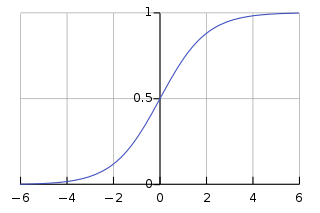
\includegraphics[width=5cm]{logistic_sigmoid.png}
\caption{Logistic sigmoid; source Wikipedia}
\end{figure}

\subsection{Cross-entropy loss}

For the binary $y$ the conditional probability distribution $p(y|\mathbf{x})$ is Bernouli with the conditional expectation $\pi = \rE(y | \mathbf{x})$. We can formulate the logistic regression problem objective as maximizing the likelihood of $\bw$ over the training set 
\begin{equation}
\max_{\bw} \prod_i^n \pi_i^{y_i} (1-\pi_i)^{1-y_i} \enspace ,
\end{equation}
where $\pi_i = \sigma(\bx_i^T \bw)$ from equation \eqref
{eq_logistic:sigmoid}.

We can instead minimize the negative log likelihood also called the \textbf{cross-entropy loss}\index{cross-entropy loss}
\begin{equation}
\min_{\bw} \sum_i^n - y_i \log \pi_i - (1-y_i) \log (1-\pi_i) \enspace ,
\end{equation}

Recall the definition of cross-entropy\index{cross-entropy}
\begin{equation}
H_p(q) = -\sum_c^C p(y_c) \log q(y_c) \enspace ,
\end{equation}
where $y$ is a random variable with C categories and $p$ and $q$ are two different distributions.

\subsection{Multi-class classification}

When we have more than 2 classes, we consider a linear model of the form $\bx^T \bw_c = z_c$ with specific parameters $\bw_c$ for each class and $z_c$ the per-class \emph{scores}\index{score}.

We can arrive at multinomial logistic regression following similar logic as in the binary case where we decompose the multiple categories $c = 1, \ldots, C$ into a set of $C-1$ dummy variables with the last category as the default pivot.

For each class we have the odds against the pivot as
\begin{equation}
\text{odds}_c = \frac{count(y=c)}{count(y = C)} = \frac{P(y=c)}{P(y =C )} = \frac{\pi_c}{\pi_C} \enspace .    
\end{equation}

The scores $z_c$ are the log-odds, the logits
\begin{equation}
z_c = \log \frac{\pi_c}{\pi_C} = \bx^T \bw_c
\end{equation}
from which we get
\begin{equation}
\pi_c = \pi_C \, \exp(\bx^T \bw_c) \qquad \text{for all } c=1, \ldots, C-1
\end{equation}


Because probabilities some to one, we have 
\begin{equation}
\pi_C = 1 - \sum_c^{C-1} \pi_c = 1 - \sum_c^{C-1} \pi_C \, \exp(\bx^T \bw_c) = 1 -  \pi_C \sum_c^{C-1} \exp(\bx^T \bw_c)
\end{equation}
and therefore 
\begin{equation}\label{eq_logistic:multinomial}
\pi_C = \frac{1}{1+\sum_c^{C-1} \exp(\bx^T \bw_c)} \qquad \pi_c = \frac{\exp(\bx^T \bw_c)}{1+\sum_c^{C-1} \exp(\bx^T \bw_c)}
\end{equation}

This is obviously equal to the binary logistic sigmoid in case of just two classes where $\pi_c =  P(y=1)$ and $\pi_C = P(y=0)$.

\paragraph{Soft-max} To get the \emph{soft-max}\index{soft-max} function instead of fixing one category as a pivot we treat all the probabilities evenly. This will in the end lead to overparametrization because we do not treat one class as the default.

As above, we have for the probabilities of each class
\begin{equation}
\pi_c = \frac{1}{Z} \, \exp(\bx^T \bw_c) \qquad \text{for all } c=1, \ldots, C \enspace ,
\end{equation}
which is now valid for all classes and where $Z$ is a common normalizing constant.

Since probability has to sum to $1$ we have
\begin{eqnarray}
1 = \sum_c^C \pi_c & = &  \frac{1}{Z} \sum_c^C \exp(\bx^T \bw_c) \nn
Z & = &   \sum_c^C \exp(\bx^T \bw_c) \nn
\pi_c & = & \frac{\exp(\bx^T \bw_c)}{\sum_c^C \exp(\bx^T \bw_c)} \enspace .
\end{eqnarray}

The coefficients in the soft-max are redundant (not uniquely identifiable), because the values of the soft-max will not change if we add a constant vector $\alpha$ to each of the parameters vector
\begin{equation}
\frac{\exp(\bx^T (\bw_c + \alpha))}{\sum_c^C \exp(\bx^T (\bw_c + \alpha))} = 
\frac{\exp(\bx^T \bw_c) \exp(\bx^T \alpha)}{\exp(\bx^T \alpha) \sum_c^C \exp(\bx^T \bw_c)} = \frac{\exp(\bx^T \bw_c)}{\sum_c^C \exp(\bx^T \bw_c)} \enspace . 
\end{equation}
If we fix $\alpha = -\bw_C$ to the parameters of the last class we get
\begin{equation}
\pi_C = \frac{\exp(\bx^T (\bw_C -\bw_C))}{\sum_c^C \exp(\bx^T (\bw_c -\bw_C))} = \frac{1}{1 + \sum_c^{C-1} \exp(\bx^T (\bw_c -\bw_C))} 
\end{equation}
and 
\begin{equation}
\pi_c = \frac{\exp(\bx^T (\bw_c -\bw_C))}{\sum_c^C \exp(\bx^T (\bw_c -\bw_C))} = \frac{\exp(\bx^T (\bw_c -\bw_C))}{1 + \sum_c^{C-1} \exp(\bx^T (\bw_c -\bw_C))} \enspace ,
\end{equation}
which is the same result as in equation \eqref{eq_logistic:multinomial} with the shifted weight vectors.


% https://en.wikipedia.org/wiki/Multinomial_logistic_regression

% https://chrisyeh96.github.io/2018/06/11/logistic-regression.html


% softmax overparametrized



%%%%%%%%%%%%%%%%%%%%%%%%%%%%%%%%%%%%%%%%%%%%%%%%%%%%%%%%%%%%%%%
%%% MG 7/8/2019 - vae log-likelihood by importance sampling %%%
%%%%%%%%%%%%%%%%%%%%%%%%%%%%%%%%%%%%%%%%%%%%%%%%%%%%%%%%%%%%%%%

\clearpage

\section{Evaluate data log likelihood by importance sampling}\index{importance sampling}

In addition to evaluting the ELBO across the test samples, it makes sense to evaluate the log-likelihood of the test data. The ELBO is formulated each time differently, depending on the graphical model etc., while the log-likelihood should be measuring always the same.

From the VAE basic assumptions we have the latent variable model
\begin{equation}
p(\bx) = \int p(\bx | \bz) p(\bz) dz \enspace , 
\end{equation}
where $p(\bz)$ is the prior for the latent $\bz$, and $p(\bx | \bz)$ is the learned conditional likelihood - the decoder of the VAE.

Hence, the log-likelihood of observation $\bx$ is 
\begin{equation}
\log p(\bx) = \log \int p(\bx | \bz) p(\bz) dz \enspace . 
\end{equation}

Empirically we could get this by sampling $\bz$ from the prior $p(\bz)$
\begin{equation}
\log p(\bx) \approx \log \sum_i^K p(\bx | \bz_i), \quad \bz_i \sim p(\bz)  \enspace . 
\end{equation}

The problem with this one is that we may need a lot of samples to get a reasonable estimate of the log-likelihood - according to the prior we may be sampling $\bz$ in an area very unlikely for any $\bx$.

Instead, adopting the importance sampling principles we may sample from the learned posterior $q(\bz|\bx)$ (the VAE decoder) so that

\begin{eqnarray}
\log p(\bx) & = & \log \int p(\bx | \bz) p(\bz) \frac{q(\bz | \bx)}{q(\bz | \bx)} dz  \nn
& = & \log \int p(\bx | \bz) q(\bz | \bx) \frac{p(\bz) }{q(\bz | \bx)} dz  
\enspace ,
\end{eqnarray}
with the empirical estimate
\begin{equation}
\log p(\bx) \approx \log \sum_i^K p(\bx | \bz_i) \frac{p(\bz_i) }{q(\bz_i| \bx)}, \quad \bz_i \sim q(\bz| \bx)  \enspace . 
\end{equation}

What we have in the loss-function (maximization of the ELBO) is the $\log$ of the probabilities. Therefore I introduce these in to the importance sampled log-likelihood
\begin{eqnarray}
\log p(\bx) 
& = & \log \int q(\bz | \bx) p(\bx | \bz) \frac{p(\bz) }{q(\bz | \bx)} dz  \nn
& = & \log \int q(\bz | \bx) \, \exp \left[ \log p(\bx | \bz)  + \log p(\bz) - \log q(\bz | \bx) \right] dz
\enspace ,
\end{eqnarray}
with the empirical estimate
\begin{eqnarray}
\log p(\bx) &\approx& \log \sum_i^K \exp \left[ \log p(\bx | \bz_i)  + \log p(\bz_i) - \log q(\bz_i | \bx) \right], \quad \bz_i \sim q(\bz| \bx) \nn
& = & \log \sum_i^K \exp \left[ \log p(\bx | \bz_i) - \log \frac{q(\bz_i | \bx)}{p(\bz_i)} \right], \quad \bz_i \sim q(\bz| \bx)
  \enspace . 
\end{eqnarray}

Here $\log \frac{q(\bz_i | \bx)}{p(\bz_i)}$ is the log probability ratio and is better evaluated in the logs as 
\begin{equation}
\log \frac{q(\bz_i | \bx)}{p(\bz_i)} = \log q(\bz_i | \bx) - \log p(\bz_i) \enspace .
\end{equation}
Note that this is the single sample empirical estimate of the KL divergence which is the same as used in the ELBO calculation in the vampprior implementation of Tomczek (though in the ELBO there it is average across multiple samples).

The first term $\log p(\bx | \bz_i)$ is simply the log conditional likelihood that is the RE part of the ELBO for a single sample $\bz$.

To evaluate the logsumexp it is safer for numerical stability to use the equivalent form
\begin{equation}
\log p(\bx) \approx a + \log \sum_i^K \exp (a_i - a) \enspace ,
\end{equation}
where 
$a_i = \log p(\bx | \bz_i) - \log \frac{q(\bz_i | \bx)}{p(\bz_i)}$ and $a = \max_i a_i$.

This is actually often already implemented in python for example in the \emph{tf.reduce\_logsumexp}.


%%%%%%%%%%%%%%%%%%%%%%%%%%%%%%%%%%%%%%%%%%%%%%%%%%%%%%%%%%%%%%%
%%% MG 7/8/2019 - vae log-likelihood by importance sampling %%%
%%%%%%%%%%%%%%%%%%%%%%%%%%%%%%%%%%%%%%%%%%%%%%%%%%%%%%%%%%%%%%%

\clearpage

\section{Some useful inequalities (or equalities) - in progress}\label{sec:Inequalities}

Some useful inequalities or equivalences found around and worth remembering.


\subsection{Numerical inequalities}\label{sec:NumericalIneq}

Based on \cite{Casella2002}.

\subsubsection{Triangle inequality}\index{Triangle inequality}
\begin{equation}\label{eq:Triangle}
|X+Y| \leq |X| + |Y|
\end{equation}

\subsubsection{Holder's inequality}\label{sec:Holder}\index{Holder's inequality}

Let $a, b > 0$ and $p, q > 1$ be any numbers satisfying
\begin{equation}\label{eq:pqPowers}
\frac{1}{p} + \frac{1}{q} = 1 \qquad p+q = pq \qquad (p-1)q = p
\end{equation}
then
\begin{equation}\label{eq:powersEq}
\frac{1}{p}a^p + \frac{1}{q}b^q \geq ab
\end{equation}
with equality only if $a^p = b^q$.

\begin{prf}
Fix $b$ and minimize the function $g(a) = \frac{1}{p}a^p + \frac{1}{q}b^q - ab$.
To minimize, we set the derivative equal to zero $d g(a) = a^{p-1} - b = 0 \Rightarrow b = a^{p-1}$. 
The value of the function at minimum is 
$\frac{1}{p}a^p + \frac{1}{q}(a^{p-1})^q - aa^{p-1} = (\frac{1}{p}-1)a^p + \frac{1}{q}a^p = 0$.
So the minimum is $0$ and \eqref{eq:powersEq} is established.
\end{prf}

We use this to get the \textbf{Holder's inequality} Let $X$ and $Y$ be two r.v. and let $p, q$ satisfy \eqref{eq:pqPowers}.
Then 
\begin{equation}\label{eq:Holders}
|\rE XY| \leq \rE |XY| \leq (\rE|X|^p)^{1/p} (\rE|Y|^q)^{1/q}
\end{equation}

\begin{prf}
The first inequality follows from the Jensen's inequality \eqref{eq:Jensens}. 
Define $a = \frac{|X|}{(\rE|X|^p)^{1/p}}$ and $b = \frac{|Y|}{(\rE|Y|^q)^{1/q}}$.
Applying \eqref{eq:powersEq} we have
\begin{align*}
\frac{1}{p}\frac{|X|^p}{\rE|X|^p} + \frac{1}{q}\frac{|Y|^q}{\rE|Y|^q} & \geq \frac{|XY|}{(\rE|X|^p)^{1/p} (\rE|Y|^q)^{1/q}} \nn
\frac{1}{p}\frac{\rE|X|^p}{E|X|^p} + \frac{1}{q}\frac{\rE|Y|^q}{\rE|Y|^q} & \geq \frac{\rE|XY|}{(\rE|X|^p)^{1/p} (\rE|Y|^q)^{1/q}} \qquad \text{(taking expectation on both sides)} \nn
1 & \geq \frac{\rE|XY|}{(\rE|X|^p)^{1/p} (\rE|Y|^q)^{1/q}} \nn
(\rE|X|^p)^{1/p} (\rE|Y|^q)^{1/q} & \geq \rE|XY| \qquad \qquad \text{QED}
\end{align*}
\end{prf}

\textbf{Cauchy-Schwarz inequality}\index{Cauchy-Schwarz inequality} is the special case of Hodler's for $p=q=2$
\begin{equation}\label{eq:CS}
|\rE XY| \leq \rE |XY| \leq (\rE|X|^2)^{1/2} (\rE|Y|^2)^{1/2}
\end{equation}

An example of CS is the \textbf{covariance inequality}\index{covariance inequality}
\begin{align}
|\rE (X-\rE X)(Y-\rE Y)| & \leq \rE |(X-\rE X)(Y-\rE Y)| \leq (\rE (X-\rE X)^2)^{1/2} (\rE (Y-\rE Y)^2)^{1/2} \nn
Cov(X,Y)^2 & \leq (\rE (X-\rE X)^2) (\rE (Y-\rE Y)^2) = \rho_X^2 \rho_Y^2
\end{align}

Another form of \textbf{covariance inequality} for two functions of a random variable states that
for $g(X), h(X)$ \textbf{both non-decreasing or both non-increasing} and therefore having $Cov(g(X)h(X)) \geq 0$
\begin{equation}
\rE(g(X)h(X)) \geq \rE g(X) \rE h(X) \enspace .
\end{equation}
For $g(X), h(X)$ \textbf{one non-decreasing the other non-increasing} and therefore having $Cov(g(X)h(X)) \leq 0$
\begin{equation}
\rE(g(X)h(X)) \leq \rE g(X) \rE h(X) \enspace .
\end{equation}

\paragraph{Other useful variants:} \

Let $Y = 1$, we get $\rE |X| \leq (\rE |X|^p)^{1/p}$ for $1 < p < \infty$.

Let $Y = 1$ and $1 < r < p < \infty$ we get $\rE |X|^r \leq (\rE |X|^{rp})^{1/p}$.

For \textbf{Liupanov's inequality}\index{Liupanov's inequality} put
$s = pr \Rightarrow 1/p = r/s$ and observe that $s > r$ so that
$1 < r < s < \infty$.
By rearranging the above we get $(\rE |X|^r)^{1/r} \leq (\rE |X|^{s})^{1/s}$.

\subsubsection{Minkowski's inequality}\label{sec:Minkowski}\index{Minkowski's inequality}

Let $X, Y$ be r.v., then for $1 \leq p < \infty$
\begin{equation}\label{eq:Minkowski}
\left(\rE |X+Y|^p\right)^{1/p} \leq \left(\rE |X|^p\right)^{1/p} + \left(\rE |Y|^p\right)^{1/p}
\end{equation}

\begin{prf}
From the triangle inequality \eqref{eq:Triangle} we have
\begin{equation*}
\rE |X+Y|^p = \rE\left(|X+Y| |X+Y|^{p-1}\right) \leq \rE\left(|X| |X+Y|^{p-1}\right) + \rE\left(|Y| |X+Y|^{p-1}\right) \enspace .
\end{equation*}
Using Hodler's to the terms on the right side we have
\begin{equation*}
\rE\left(|X| |X+Y|^{p-1}\right) \leq (\rE |X|^p)^{1/p} (\rE |X+Y|^{q(p-1)})^{1/q}
\end{equation*}
with $p,q$ satisfying \eqref{eq:pqPowers} and therefore
\begin{align*}
\rE |X+Y|^p & \leq (\rE |X|^p)^{1/p} \left(\rE |X+Y|^{q(p-1)}\right)^{1/q} + (\rE |Y|^p)^{1/p} \left(\rE |X+Y|^{q(p-1)}\right)^{1/q} \\
\frac{\rE |X+Y|^p}{\left(\rE |X+Y|^{q(p-1)}\right)^{1/q}}
& \leq (\rE |X|^p)^{1/p} + (\rE |Y|^p)^{1/p} \\
\left(\rE |X+Y|^{p}\right)^{1 - 1/q}
& \leq (\rE |X|^p)^{1/p} + (\rE |Y|^p)^{1/p} \qquad q(p-1) = p \text{ from \eqref{eq:pqPowers}} \\
\left(\rE |X+Y|^{p}\right)^{1/p}
& \leq (\rE |X|^p)^{1/p} + (\rE |Y|^p)^{1/p} \qquad \qquad \text{QED}
\end{align*}
\end{prf}

\subsection{Optimization}\label{sec:Optimization}

\subsubsection{Change max to min}\index{max to min}

\begin{equation}
\min f(x) = - \max -f(x)
\end{equation}

\begin{prf}
$m \leq f(x)$ for any $f(x)$ is the minimum.
We know that $-m \geq -f(x)$ which tells us that $-m$ is the maximum of $-f(x)$, that is $- m = \max - f(x)$.
Multiplying both sides by $-1$ we get the result.
\end{prf}

\subsubsection{Min of monotonic function}

For a non-decreasing function $f$ we have $\max f(x) = f(\max x)$.

\begin{prf}
If $f$ is non-decreasing then for all $x \geq x'$ we have $f(x) \geq f(x')$.
For $\max f(x) = f^* = f(x^*)$ we know that $f(x^*) \geq f(x)$ and therefore
$x^* \geq x$ for any $x$ which gives $x^* = \max x$ and therefore $\max f(x) = f(\max x)$.
\end{prf}


\subsubsection{Min of exponential}

Using the previous results we have ($\exp$ is monotonically increasing)
\begin{equation}\label{eq:MinExp}
\min \exp( - a) = \exp (\min -a) = \exp (- \max a)
\end{equation}

\subsubsection{Jensen's inequality}\index{Jensen's inequality}

A function $f$ is convex\index{convex function} if for all $x_1, x_2 \in \mX{}$ and all $t \in [0,1]$ we have
\begin{equation}\label{eq:ConvexDef}
f(tx_1 + (1-t)x_2) \leq t f(x_1) + (1-t)f(x_2)
\end{equation}
In words, convex function of an average of two points is below the average of the function evaluations at the two points.

This can be extended from averages to expectations for a convex function $f$ (e.g. $\exp$)
\begin{equation}\label{eq:Jensens}
f(\rE{X}) \leq \rE{f(X)} \enspace .
\end{equation}

For a concave function $g$ (e.g. $\log$) the inequality reverses into
\begin{equation}
g(\rE{X}) \geq \rE{g(X)} \enspace .
\end{equation}


\subsection{Basic probability}\label{sec:BasicProb}

\subsubsection{Union bound}\index{union bound}

Based on \cite{Casella2002}.

For a countable set of events $A_1, A_2, \ldots, A_n$ we have
\begin{equation}
\rP (\cup_i^n A_i) \leq \sum_i^n \rP (A_i)
\end{equation}

\begin{prf}
From the basic laws of probability we have $\rP(A \cup B) = \rP(A) + \rP(B) - \rP(A \cap B) \leq \rP(A) + \rP(B)$.
We indicate by $A = \cup_i^{n-1} A_i$ and $B = A_n$ to get
\begin{equation}
\rP (\cup_i^n A_i) = \rP(\cup_i^{n-1} A_i \cup A_n) \leq \rP(\cup_i^{n-1} A_i) + \rP(A_n)
\end{equation}
from which by induction we get the result.
\end{prf}

\subsection{Variable transformation}\label{sec:VarTransform}\index{variable transformation}

Based on \cite{random}.

We have a r.v. $X$ taking values in a set $S$ with a known probability distribution $\rP$.

A function $g: S \to T$ is a new r.v. $Y = g(X)$ with values in $T$.

For $B \subseteq T$, $g^{-1}(B) = \{x \in S: g(x) \in B\}$ is the \emph{inverse image}\index{inverse image} (preimage)\index{preimage} of $B$ under $g$ and the probability is $P(Y \in B) = P(g(X) \in B) = P(X \in g^{-1}(B))$. 

If the function $g(x) = y$ is \textbf{one-to-one} than it has an inverse \emph{function} $g^{-1}(y) = x$ which is as well one-to-one.

If $g(x) = y$ is \textbf{strictly increasing} then the cumulative distribution function is
\begin{equation}
G(y) = P(Y \leq y) = P(g(X) \leq g(x)) = P(X \leq x) = F(x) \enspace ,
\end{equation}
where $F$ is the cdf of X and $x = g^{-1}(y)$.

If $g(x) = y$ is \textbf{strictly decreasing} then
\begin{equation}
G(y) = P(Y \leq y) = P(g(X) \leq g(x)) = P(X \geq x) = 1 - F(x) \enspace .
\end{equation}


However, if the function $g(x) = y$ is \textbf{many-to-one} than it does not have an inverse \emph{function}, and $g^{-1}(y) = \{ x_1, x_2, \ldots \}$ is the one-to-many inverse image. In the general case, we cannot make similar claims about cdf (or pdf) of Y as above.

Still, for a \textbf{non-decreasing} function $g(x) = y$ with an inverse image $g^{-1}(y) = (x_1, x_2), \ x_1 \leq x_2$ we have
\begin{eqnarray}
\text{case 1} \quad G(y) = P(Y \leq y) = P(g(X) \leq g(x_1)) & > & P(X \leq x_1) = F(x_1) \nn
\text{case 2} \quad G(y) = P(Y \leq y) = P(g(X) \leq g(x_2)) & = & P(X \leq x_2) = F(x_2) \nn
\text{in general} \quad G(y) = P(Y \leq y) = P(g(X) \leq g(x)) & \geq & P(X \leq x) = F(x) \nn
& \text{and} & \\
\text{case 1} \quad 1 - G(y) = P(Y \geq y) = P(g(X) \geq g(x_1)) & = & P(X \geq x_1) = 1 - F(x_1) \nn
\text{case 2} \quad 1 - G(y) = P(Y \geq y) = P(g(X) \geq g(x_2)) & > & P(X \geq x_2) = 1 - F(x_2) \nn
\text{in general} \quad 1 - G(y) = P(Y \geq y) = P(g(X) \geq g(x)) & \geq & P(X \geq x) = 1 - F(x) \nonumber
\end{eqnarray}

\begin{table}[h!]
\caption{Example of probability distribution of a non-decreasing variable transformation $g(x)$.}
\label{tab:VarTransform}
\vskip 0.15in
\begin{center}
\begin{tabular}{cccc | cccc}
\hline
$x$ & $P(X=x)$  & $P(X \leq x)$ & $P(X \geq x)$ & $g(x)$ & $P(g(X)=g(x))$ & $P(g(X) \leq g(x))$ & $P(g(X) \geq g(x))$ \\
\hline
1    & 1/6 & 1/6 & 1 &\multirow{2}{*}{2} & \multirow{2}{*}{1/3} & \multirow{2}{*}{1/3} & \multirow{2}{*}{1}\\
2    & 1/6 & 1/3 & 5/6 \\
\hline
3    & 1/6 & 1/2 & 2/3 &\multirow{2}{*}{4} & \multirow{2}{*}{1/3} & \multirow{2}{*}{2/3} & \multirow{2}{*}{2/3}\\
4    & 1/6 & 2/3 & 1/2 \\
\hline
5    & 1/6 & 5/6 & 1/3 &\multirow{2}{*}{6} & \multirow{2}{*}{1/3} & \multirow{2}{*}{1} & \multirow{2}{*}{1/3}\\
6    & 1/6 & 1 & 1/6 \\
\hline
\end{tabular}
\end{center}
\end{table}





\subsection{Concentration bounds}\label{sec:concentrationBounds}

Based on \cite{Boucheron2013}.

By concentration inequality we usually mean an upper bound for the probability that a r.v. $Z$ differs from its expected value by more than some amount $t > 0$. That is we seek upper bounds on the probabilities in the form
\begin{equation}
\rP{(Z-\rE{Z} \geq t)} \quad \text{ and } \quad \rP{(Z-\rE{Z} \leq -t)}
\end{equation}
or equivalently on the probability
\begin{equation}
\rP{(|Z-\rE{Z}| \geq t)} \enspace .
\end{equation}

\subsubsection{Markov's inequality}\index{Markov's inequality}

Based on \cite{Casella2002}.

For a non-negative random variable $Y$, i.e. $\rP(Y < 0) = 0$, and all $t > 0$ we have
\begin{equation}\label{eq:Markov}
\rP(Y \geq t) \leq \frac{\rE Y}{t}
\end{equation}

By fixing $t = r \, \rE Y$ we get the equivalent
\begin{equation}
\rP(Y \geq r \, \rE Y) \leq \frac{1}{r}
\end{equation}

\begin{prf}
Following \cite{Casella2002}. For a given $t > 0$ it holds that 
\begin{eqnarray*}
t \, \ind(Y \geq t) & \leq & Y \ \quad \ (\ind(Y \geq t) = 1 \text{ if } Y \geq t \text{ and 0 otherwise})\\
\rE (t \,\ind(X \geq t)) & \leq & E Y \quad \text{(by monotonicity of expectation)} \\
t \, \big( 1 \, \rP(Y \geq t) + 0 \, \rP(Y < t) \big) & \leq & \rE Y  \quad \text{(expanding the expectation)} \\
\rP(Y \geq t) & \leq & \frac{\rE Y}{t} \quad \text{QED}
\end{eqnarray*}
\end{prf}

We can apply \eqref{eq:Markov} to a non-negative random function $Y = g(Z)$ of r.v. $Z$ taking values in $I \subseteq \mR$ so that 
\begin{equation}
\rP(g(Z) \geq t) \leq \frac{\rE g(Z)}{t}
\end{equation}
and for non-decreasing nonnegative $g$ with $Z, t \in I \subseteq \mR$ so that $g(t) > 0$
\begin{equation}\label{eq:MarkovFunc}
\rP(Z \geq t) \leq \rP(g(Z) \geq g(t)) \leq \frac{\rE g(Z)}{g(t)}
\end{equation}

\subsubsection{Chebyshev's inequality}\index{Chebyshev's inequality}

Based on \cite{Boucheron2013}.

Taking $g(t) = t^2$ and $Y = |Z - \rE{Z}|$, we get from \eqref{eq:MarkovFunc}
\begin{eqnarray}\label{eq:Chebyshev}
\rP(|Z - \rE{Z}|^2 \geq t^2) & \leq & \frac{\rE (|Z - \rE{Z}|^2)}{t^2} \nn
\rP(|Z - \rE{Z}| \geq t) & \leq & \frac{Var \, Z}{t^2}
\end{eqnarray}

More generally, we may take $g(t) = t^q$ for some $q>0$ and all $t>0$ to get the general \textbf{moment bounds}\index{moment bounds}
\begin{eqnarray}\label{eq:momentBound}
\rP(|Z - \rE{Z}| \geq t) & \leq & \frac{\rE (|Z - \rE{Z}|^q)}{t^q}
\end{eqnarray}
and we may choose $q$ to optimize the upper bound. 

Nevertheless, variance (that is $q = 2$) is probably the easiest to handle.

For a \textbf{sum of independent} r.v. $Z = \sum_i^n X_i$ we have for the expectation $\rE{Z} = \sum_i^n \rE{X_i}$, for the variance $Var Z = \sum_i^n Var X_i$ and therefore from \eqref{eq:Chebyshev}
\begin{eqnarray}\label{eq:ChebyshevSum}
\rP\left(\Big| \sum_i^n X_i - \rE{\sum_i^n X_i} \Big| \geq t\right) & \leq & \frac{Var \, \sum_i^n X_i}{t^2} \nn
\rP\left(\Big| \sum_i^n (X_i - \rE{X_i}) \Big| \geq t\right) & \leq & \frac{\sum_i^n Var X_i}{t^2} \nn
\rP\left(\frac{1}{n} \Big| \sum_i^n (X_i - \rE{X_i}) \Big| \geq \frac{t}{n}\right) & \leq & \frac{\sum_i^n Var X_i}{t^2} \nn
\rP\left(\frac{1}{n} \Big| \sum_i^n (X_i - \rE{X_i}) \Big| \geq r \right) & \leq & \frac{n^{-1} \sum_i^n Var X_i}{n r^2} \qquad \frac{t}{n} = r, \ t^2 = r^2n^2
\end{eqnarray}

\subsubsection{Cramer-Chernoff method}\index{Cramer-Chernoff method}

Based on \cite{Boucheron2013}.

For r.v. $Z \in \mR$ and $g(t) = e^{\lambda t}$ where $\lambda > 0$ we get from Markov's \eqref{eq:MarkovFunc}
\begin{equation}\label{eq:MarkovExp}
\rP(Z \geq t) \leq \frac{\rE e^{\lambda Z}}{e^{\lambda t}} \enspace ,
\end{equation}
where $F(\lambda) = \rE e^{\lambda Z}$ is the \emph{moment generating function}\index{moment generating function} (in general defined for all $\lambda \in \mR{}$).
We will optimize for $\lambda \geq 0$ to get the best possible concentration bound.

Define $\psi_Z(\lambda) := \log \rE e^{\lambda Z}$ for all $\lambda \geq 0$ and introduce \emph{Cramer transform}\index{Cramer transform} of $Z$
\begin{equation}\label{eq:CramerTransform}
\psi_Z^*(t) = \sup_{\lambda \geq 0}(\lambda t - \psi_Z(\lambda))
\end{equation}

From \eqref{eq:MarkovExp} we get the \textbf{Chernoff's inequality}\index{Chernoff's inequality}
\begin{equation}\label{eq:Chernoff}
\rP(Z \geq t) \leq \exp (- \psi_Z^*(t))
\end{equation}

\begin{prf}{Chernoff's inequality}
\begin{eqnarray*}
\rP(Z \geq t) & \leq & e^{-\lambda t}\rE e^{\lambda Z} =
\exp \log (e^{-\lambda t}\rE e^{\lambda Z}) =
\exp (\psi_Z(\lambda) - \lambda t) \nn
\rP(Z \geq t) & \leq & \min_\lambda \exp (\psi_Z(\lambda) - \lambda t)  \qquad  \qquad (\text{true for any } \lambda \geq 0 \text{ so also for } \min) \nn
\rP(Z \geq t) & \leq & \exp (- \max \lambda t - \psi_Z(\lambda)) = \exp (- \psi_Z^*(t)) \qquad (\text{use } \eqref{eq:MinExp}) \qquad \text{QED}
\end{eqnarray*}
\end{prf}

For $\lambda = 0$ we have $\psi_Z(0) := \log \rE e^{0 Z} = \log 1 = 0$ and hence (as we can always opt for $\lambda = 0$ if there is no better $\lambda$)
\begin{equation}\label{eq:cramer_positive}
\psi_Z^*(t) = \sup_{\lambda \geq 0}(\lambda t - \psi_Z(\lambda)) \geq 0
\end{equation}

By Jensen's inequality \eqref{eq:Jensens} we have $\psi_Z(\lambda) := \log \rE e^{\lambda Z}$.
Therefore for \textbf{negative} $\lambda < 0$ we get for all $t \geq \rE{Z}$ 
\begin{eqnarray}
t &\geq& \rE{Z} \nn
\lambda t &\leq& \lambda \rE{Z} \qquad (\lambda < 0) \nn
\lambda t &\leq& \psi_Z(\lambda) \qquad (\log \rE e^{\lambda Z} \geq \rE \log e^{\lambda Z} = \lambda \rE Z)\nn
\lambda t - \psi_Z(\lambda) &\leq& 0
\end{eqnarray}

For all $t \geq \rE{Z}$ we can therefore extend the supremum in \eqref{eq:CramerTransform} over $\lambda \in \mR$ because none of the $\lambda < 0$ will be considered due to \eqref{eq:cramer_positive}.
\begin{equation}\label{eq:FenchelTransform}
\psi_Z^*(t) = \sup_{\lambda \in \mR}(\lambda t - \psi_Z(\lambda))
\end{equation}
which is known as the \emph{Fenchel-Legendre transform}\index{Fenchel-Legendre transform} or as the \emph{convex conjugate}\index{convex conjugate} of $\psi_Z(\lambda)$.

Chernoff's inequality is trivial if $\psi_Z^*(t) = 0$ (simply $\rP(Z \geq t) \leq 1$). This happens whenever $\psi_Z(\lambda) = \infty$ for all positive $\lambda > 0$ or if $t \leq \rE{Z}$.

\begin{prf}
If $t \leq \rE{Z}$ and $\lambda \geq 0$ then
\begin{eqnarray*}
t &\leq& \rE{Z} \nn
\lambda t &\leq& \lambda \rE{Z} \leq \psi_Z(\lambda) \qquad (\lambda > 0) \nn
\lambda t - \psi_Z(\lambda) &\leq& 0 \qquad \text{QED}
\end{eqnarray*}
\end{prf}

To avoid the trivial situation, we assume that there exists $\lambda > 0$ such that $\rE e^{\lambda Z} \leq \infty$.
Denote by $b$ the supremum of the interval of such $\lambda$ so that $0 < b < \infty$.
Then $\psi_Z(\lambda)$ is convex and infinitely many times differentiable on $I=(0,b)$ (strictly convex if $Z$ is not almost surely constant).

\begin{prf} of convexity using convex function definition \eqref{eq:ConvexDef} and Holder's inequality \eqref{eq:Holders} with $X = e^{t\lambda_1 Z}$, $Y = e^{(1-t)\lambda_2 Z}$ and $p = 1/t$ and $q = 1/(1-t)$.

\begin{align*}
\rE e^{t\lambda_1 Z} e^{(1-t)\lambda_2 Z} & \leq \left(\rE e^{\lambda_1 Z}\right)^t \left(\rE e^{\lambda_2 Z}\right)^{1-t} \\
\log \rE e^{[t\lambda_1 + (1-t)\lambda_2] Z} & \leq t \log \rE e^{\lambda_1 Z} + (1-t) \log \rE e^{\lambda_2 Z} \qquad \text{QED}
\end{align*}
\end{prf}

The differentiability means that the Cramer transform $\psi_Z^*(t)$ can be obtained by differentiating$ \lambda t - \psi_Z(\lambda)$ with respect to $\lambda$ to get
\begin{equation}
\psi_Z^*(t) = \lambda_t t - \psi_Z(\lambda_t) \enspace ,
\end{equation}
where $\lambda_t$ is such that $t = \psi'_Z(\lambda_t)$.

Because $\psi_Z(\lambda)$ is convex the derivative $\psi'$ and its inverse $(\psi')^{-1}$ are increasing.
We get $\lambda_t = (\psi')^{-1}(t)$.

\begin{example}
For a \textbf{centred normal random variable} $Z$ with variance $\sigma^2$ and the mgf
$\rE e^{\lambda Z} = e^{\sigma^2 \lambda^2/2}$ we have $\psi_Z(\lambda) = \sigma^2 \lambda^2/2$,
$\psi'_Z(\lambda) = \sigma^2 \lambda$ and therefore $\lambda_t = t/\sigma^2$.

For every $t > 0$, 
\begin{equation}
\psi_Z^*(t) = \lambda_t t - \psi_Z(\lambda_t) = \frac{t^2}{\sigma^2} - \frac{\sigma^2 t^2}{2 \sigma^4} =  \frac{t^2}{2\sigma^2}
\end{equation}
so that the Chernoff's inequality \eqref{eq:Chernoff} in this case gives
\begin{equation}
\rP(Z \geq t) \leq e^{- t^2/(2\sigma^2)}
\end{equation}
\end{example}


\paragraph{Sums of independent random variables}
Though Chernoff's inequality may not be as sharp as the moment bounds \eqref{eq:momentBound}, it is particularly convenient for sums of independent random variables.

For a \textbf{sum of independent} r.v. $Z = \sum_i^n X_i$ we have for the moment generating function
\begin{equation}
\rE e^{\lambda Z} = \rE e^{\lambda \sum_i^n X_i} = \rE \prod_i^n e^{\lambda X_i} = \prod_i^n \rE e^{\lambda X_i}
\end{equation}
and therefore 
\begin{equation}
\psi_Z(\lambda) = \log \rE e^{\lambda Z} = \log \prod_i^n \rE e^{\lambda X_i} = \sum_i^n \log \rE e^{\lambda X_i} = n \psi_X(\lambda)
\end{equation}

\begin{equation}
\psi_X^*(t) = \lambda_t t - \psi_X(\lambda_t) \enspace ,
\end{equation}
where $\lambda_t$ is such that $t = \psi'_X(\lambda_t)$.

\begin{equation}
\psi_Z^*(t) = \lambda_t t - n \psi_X(\lambda_t) \enspace ,
\end{equation}
where $\lambda_t$ is such that $t = n \ \psi'_X(\lambda_t)$ so that
\begin{equation}
\psi_Z^*(t) = n \psi_X^*\left(\frac{t}{n}\right) 
\end{equation}


\subsection{Sub-Gaussian random variables}\label{sec:SubGaussian}\index{Sub-Gaussian random variables}
Many r.v. have tail probabilities decreasing at least as rapidly as Gaussian r.v.

\begin{definition}[sub-Gaussian r.v.]
A centered r.v. $X$ is said to be sub-Gaussian with variance factor $\nu$ (bound on the variance of $X$) if its $\log$ mgf is
\begin{equation}
\psi_X(\lambda) \leq \frac{\lambda^2 \nu}{2}
\end{equation}
We denote the collection of such r.v. by $\mG(\nu)$.
\end{definition}
In other words, $X$ belongs to $\mG(\nu)$ if its mgf is dominated by that of a centered Gaussian r.v. with variance $\nu$.
If independent r.v. $X_1, \ldots, X_n$ are all sub-Gaussian $X_i \leq \mG(\nu_i)$ then $\sum_i X_i \in \mG \left(\sum_i^n \nu_i\right)$.

\paragraph{Other properties:}

From Chernoff's inequality, if $X$ belongs to $\mG(\nu)$ then for every $t > 0$ (see the Gaussian example)
\begin{equation}
\rP(X > t) \lor \rP(-X > t) \leq e^{- t^2/(2\nu)} \enspace ,
\end{equation}
where $a \lor b$ denotes the maximum of $a$ and $b$.

\begin{theorem}
Let $X$ be r.f. with $\rE X = 0$. If for some $\nu > 0$ 
\begin{equation*}
\rP(X > x) \lor \rP(-X > x) \leq e^{- t^2/(2\nu)} \qquad \text{for all } x > 0
\end{equation*}
then for every integer $q \geq 1$
\begin{equation}\label{eq:bound_esauared}
\rE X^{2q} \leq 2q!(2\nu)^q \leq q!(4\nu)^q \enspace .
\end{equation}
Conversely, if for some constant $C > 0$
\begin{equation*}
\rE X^{2q} \leq q!(C)^q
\end{equation*}
then $X \in \mG(4C)$ (sub-Gaussian with $\nu = 4C$).
\end{theorem}


\begin{prf}
Wlg we may assume $\nu = 1$ because otherwise we can apply a simple transformation $X / \sqrt{v}$.
With $q \geq 1$, the random variable $Y = X^2q = |X|^2q \geq 0$ is \textbf{nonnegative}.

\begin{theorem}[Fubini's]\index{Fubini's theorem}
For a product probability space $(S \times T, \mS \otimes \mT, \mu \otimes \nu)$ and $f : S \times T \to \mR$ measurable, the integral with respect to the product measure $(\mu \otimes \nu)$ is equivalent to the iterated integrals
\begin{equation}
\int_{S \times T} f(x,y) d(\mu \otimes \nu)(x,y) = \int_{S} \int_{T} f(x,y) d \nu(y) d \mu(x) = 
\int_{T} \int_{S} f(x,y) d \mu(x) d \nu(y)
\end{equation}
\end{theorem}

For nonnegative $Y$ we have 
\begin{align*}
\int_0^\infty \rP(Y \ge y) dy & = \int_0^\infty \int_y^\infty p(t) dt \, dy \qquad \text{(definition of density)}\\
& = \int_0^\infty \int_0^y p(t) dy \, dt \qquad \text{(swap integrals }, \infty > y > 0, \infty > t > y, \Rightarrow \infty > t > 0, t > 0 > 0)\\
& = \int_0^\infty [y \, p(t)]_0^t \, dt \qquad \text{(integral of constant)}\\
& = \int_0^\infty t \, p(t) \, dt = \rE Y
\end{align*}

Therefore 
\begin{align*}
\rE X^{2q} & = \int_0^\infty \rP(|X|^{2q} \ge x) dx \\
& = \int_0^\infty \rP(|X| \ge x^{1/(2q)}) dx
\end{align*}
Substitute
\begin{align*}
u & = x^{1/(2q)} & du & = 1/(2q) \, x^{1/(2q)-1} \, dx \\
u^{2q} & = x & 2q \, du & = \frac{x^{1/(2q)}}{x} \, dx \\
 & & 2q \, du & = \frac{u}{u^{2q}} \, dx \\
 & & 2q \, u^{2q-1} du & = dx 
\end{align*}
and continue from above
\begin{align*}
\rE X^{2q} 
& = \int_0^\infty \rP(|X| \ge x^{1/(2q)}) dx \\
& = \int_0^\infty 2q \, u^{2q-1} \rP(|X| \ge u) du \\
& = \int_0^\infty 2q \, u^{2q-1} \big(\rP(X \ge u) + \rP(-X \ge u)\big) du \\
& \leq 4q \, \int_0^\infty u^{2q-1} e^{- u^2/(2\nu)} du
\end{align*}
Substitute
\begin{align*}
u & = \sqrt{2t\nu} & du & = \sqrt{2\nu}  \, \frac{1}{2} t^{-0.5} \, dt \\
\frac{u^{2}}{2\nu} & = t & 2 \, du & = 1/u \, dt \\
 & & 2u \, du & = dt \\
\end{align*}
and continue from above
\begin{align*}
\rE X^{2q} 
& \leq 4q \, \int_0^\infty u^{2q-1} e^{- u^2/(2\nu)} du \\
& = 4q \, \int_0^\infty (2t\nu)^{q-0.5} e^{-t}\sqrt{2\nu}  \, \frac{1}{2} t^{-0.5} \, dt \\
& = 4q \, \int_0^\infty 2^{q-0.5+0.5-1} \nu^{q-0.5+0.5} t^{q-0.5 -0.5} e^{-t} dt \\
& = 2^{q+1} q \, \nu^{q}  \int_0^\infty t^{q-1} e^{-t} dt \\
& = 2^{q+1} q \, \nu^{q}  (q-1)! \qquad \href{https://en.wikipedia.org/wiki/List\_of\_integrals\_of\_exponential\_functions}{\text{(wiki, intergrals of exp func)}}\\
& = 2^{q+1} \, \nu^{q}  q! = 2 q! \, (2 \nu)^q \leq  q! \, (4 \nu)^q \qquad \text{QED } \eqref{eq:bound_esauared}
\end{align*}


\end{prf}



\begin{thebibliography}{9}

\bibitem{Casella2002}
Casella, G., Berger, R. L.: Statistical Inference. Duxbury. 2002

\bibitem{Boucheron2013}
Boucheron, Stéphane, Gábor Lugosi, and Pascal Massart. Concentration Inequalities: A Nonasymptotic Theory of Independence. Oxford University Press, 2013.

\bibitem{random} Kyle Siegrist, Random website, https://www.randomservices.org/random/

\bibitem{Mohri2012}
Mohri, M., Rostamizadeh, A., \& Talwalkar, A.: Foundations of Machine Learning. MIT Press (2012)

\end{thebibliography}




% print index
\phantomsection
\cleardoublepage
\addcontentsline{toc}{section}{\indexname}
\printindex

\end{document}
%%% Local Variables:
%%% mode: latex
%%% TeX-master: t
%%% End:
